\begin{frame}{Structure of the course}
    \begin{itemize}
        \item \alert{Moodle:} \url{https://go.epfl.ch/error-control}
        \vspace{0.5em}
        \item Lectures split into two rough segments
            \begin{itemize}
                \vspace{-0.3em}
                \item \alert{First half:} Matrix eigenvalue problems \& floating-point error
                \vspace{-0.3em}
                \item \alert{Second half:} Operator theory \& discretisation error
            \end{itemize}
        \vspace{0.5em}
        \item Attendance of exercises is \alert{expected} \textcolor{grey5}{(introduces new material!)}
        \vspace{0.5em}
        \item Evaluation:
            \begin{itemize}
                \vspace{-0.3em}
                \item 4 marked problem sheets \textcolor{grey5}{($1/3$ of grade)}
                \vspace{-0.3em}
                \item 2 projects \textcolor{grey5}{($2/3$ of grade)}
                \vspace{-0.3em}
                \item Both done in \alert{teams of $2$ students}.
                \vspace{-0.3em}
                \item Interdisciplinary teams are highly recommended
            \end{itemize}
        \vspace{0.5em}
        \item Working on the sheets and the projects
            \alert{requires substantial time outside class}
            \begin{itemize}
                \vspace{-0.3em}
            \item[$\Rightarrow$] We will setup \alert{survey} in week 2 to \alert{aid formation of groups}
            \end{itemize}
    \end{itemize}
\end{frame}

\begin{frame}{Details on the problem sheets}
    \begin{itemize}
        \item One sheet per week from moodle: \url{https://go.epfl.ch/error-control}
        \vspace{1em}
        \item Only 4 sheets are handed in \& marked:
            \begin{itemize}
                \vspace{-0.3em}
                \item Deadline Friday 12:00 the next week
            \end{itemize}
        \vspace{1em}
        \item Namely \textcolor{grey5}{(tentatively)} the sheets of
            \begin{itemize}
                \vspace{-0.3em}
                \item Week 2 \textcolor{grey5}{(28th Sept)}, deadline \textbf{6th Oct}
                \vspace{-0.3em}
                \item Week 3 \textcolor{grey5}{(5th Oct)}, deadline \textbf{13th Oct}
                \vspace{-0.3em}
                \item Week 5 \textcolor{grey5}{(19th Oct)}, deadline \textbf{27th Oct}
                \vspace{-0.3em}
                \item Week 6 \textcolor{grey5}{(26th Oct)}, deadline \textbf{3rd Nov}
            \end{itemize}
        \vspace{1em}
        \item General guideline: Each member of the group obtains the same mark on each sheet
    \end{itemize}
\end{frame}

\begin{frame}{Details on the projects}
    \smaller
    \begin{itemize}
        \item Each project is essentially a larger problem sheet
        \item One joint solution is submitted by each group
        \item Responsibilities should be shared equally.
        \vspace{0.5em}
        \item In the week after submission:
            \begin{itemize}
                \smaller
                \item Individual interviews of ca.~15 minutes on the submission
                \item \alert{Content:} The solution submitted by the group
            \end{itemize}
        \vspace{0.5em}
        \item Evaluation criteria:
            \begin{itemize}
                \smaller
                \item Soundness of the submitted solution
                \item Clarity and structure of the notebook
                \item Presentation of the results as part of the interview
                \item Ability to answer questions in the interview
            \end{itemize}
        \vspace{0.5em}
        \item Each group member obtains an \alert{individual} mark.
    \end{itemize}
\end{frame}

\begin{frame}{Topics of the projects}
    \begin{itemize}
        \item Project 1: \alert{Numerical investigation of quantum tunnelling}
            \begin{itemize}
                \vspace{-0.5em}
                \item Handout: 2nd November \textcolor{grey5}{(tentative)}
                \vspace{-0.5em}
                \item Duration: 4 weeks, i.e.~projected deadline: \textbf{30th November}
            \end{itemize}
        \vspace{1.0em}
        \item Project 2: \alert{Band structures with guaranteed error bars}
            \begin{itemize}
                \vspace{-0.5em}
                \item Handout: 30th November \textcolor{grey5}{(tentative)}
                \vspace{-0.5em}
                \item Duration: 6 weeks, i.e.~projected deadline: \textbf{11th January}
            \end{itemize}
        \vspace{0.5em}
        \begin{center}
        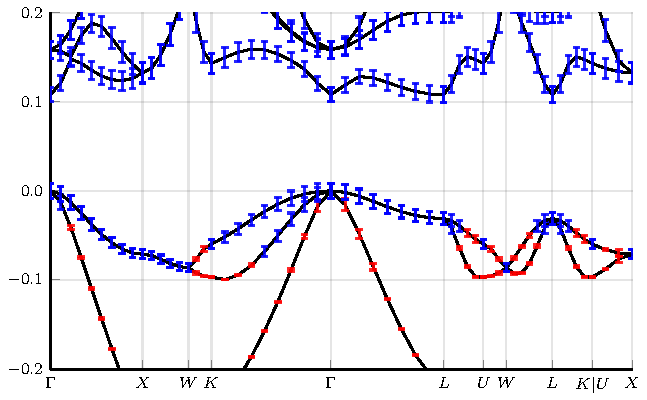
\includegraphics[width=0.5\textwidth]{img/si_band_errors.pdf}
        \end{center}
    \end{itemize}
\end{frame}

\begin{frame}{Questions ?}
    \begin{center}
        \huge{Questions ?}
    \end{center}
\end{frame}
